\section{Design pattern}

Afin d'obtenir un code modulaire et facilement extensible nous avons mis en
œuvre divers patrons de conception au cours de ce projet. Le premier est le
\emph{design pattern Singleton} que nous avons utilisé à chaque fois que nous
voulions nous assurer qu'une classe n'était instanciée qu'une seule fois. Le
second est le \emph{design pattern Factory} qui nous a servi lorsqu'il était
nécessaire de contrôler et d'abstraire la création de multiples objets.

\subsection{Singleton}

\paragraph{}
À plusieurs reprises nous avons créé des classes étant des singletons et pour
diverses raison. Notamment lorsque nous voulions qu'une classe fournisse un
ensemble cohérent d'outils aux autres classes de notre projet, tout en
maintenant un état, l'utilisation d'un singleton nous a semblé naturel. En
effet, il ne serait pas pertinent dans ce cas que chaque classe voulant
utiliser les fonctionnalités offertes par la classe outil doive instancier un
objet de cette dernière ; cela provoquerait un surcoût mémoire car il y aurait
plusieurs instances en mémoire là où une seule est suffisante ; on aurait
également un surcoût en temps de calcul à chaque instanciation d'un nouvel
objet alors que la classe singleton ne paie se coût qu'une seule fois puis
fourni directement la référence de l'objet créé les fois suivantes. Enfin
chaque instance aurait son propre état et il serait plus compliqué de
maintenir un état cohérent sur tout le projet.

\paragraph{}
Les avantages décrits ici de la classe singleton seraient également offert par
une classe statique, cependant nous avons préféré opter pour le premier choix
respectant les principes de la programmation orientée objet. De plus les
singletons sont plus flexibles et offrent un meilleur contrôle de leur
initialisation.

\subsubsection{Fichier de configuration}

\paragraph{}
Une des classes respectant ce patron de conception est la classe
\verb!WorldConfig! qui s'appuie sur un fichier de configuration pour fournir
les valeurs de nombreux paramètres à l'ensemble des autres classes.

\paragraph{}
Typiquement ici l'utilisation d'un singleton plutôt qu'une classe statique
nous permet d'assurer que l'ensemble des initialisations du projet sont
effectuées avant d'effectuer l'initialisation de cette classe qui va lire et
parser le fichier de configuration.

\paragraph{}
Ce fichier de configuration (\verb!world.cfg! localisé aux côtés des fichiers
binaire) offre un contrôle de nombreux paramètres du projet (tel que le nombre
d'agents au départ, la taille du terrain, les meshes à utiliser pour chaque
agent ou encore des paramètres de comportement) et évite d'avoir à recompiler
le projet pour modifier le moindre de ces paramètres.


\subsection{Factory}
\paragraph{}
Dans ce projet nous avons définit un agent comme étant (de façon simplifiée)
un mesh ayant un comportement. Pour cette raison, la création d'un agent
requiert de spécifier le mesh à utiliser et le comportement.

\paragraph{}
Afin de simplifier la création des agents, nous avons utilisé le \emph{design
pattern Factory}. Il en existe de plusieurs sortes et nous nous en sommes
inspiré pour améliorer la flexibilité et la maintenabilité de notre
code. Ces \emph{Factories} gèrent à la fois la création d'objets - agents ou
items - et la propagation de mises à jour à ces objets. Grâce à ce design,
l'affectation d'un comportement à un agent est facilement contrôlable par un
utilisateur (via la factory correspondante dans \verb!AgentFactory!), elle
n'est pas écrite "en dur" dans la définition de chaque type d'agent. De plus
l'affectation d'un nouveau comportement à un type d'agent requiert de ne
changer qu'une seule ligne de code - au niveau de la définition de la factory
- et non pas de changer chaque appel au constructeur d'un agent en spécifiant
le nouveau comportement à utiliser.

\paragraph{}
On remarquera qu'il n'est pas possible de créer des ogres constructeurs et
d'autres ogres destructeurs en utilisant les factories. Cependant, cela ne
fait pas partie des besoins du projet et cela reste possible en créant les
agents sans passer par la factory - bien que l'on perde alors les avantages
décrits ci-dessus.

\section{Architecture}
Nous sommes partis d'un projet vierge afin de comprendre l'intégralité du code
utilisé. Au cours du projet, nous nous sommes inspirés des tutoriels
disponibles.

Nous avons repris l'idée de la classe \texttt{OgreApp} qui regroupe l'ensemble
des fonctions nécessaires aux bons fonctionnements d'une application ogre. On
trouve donc les fonctions pour charger les ressources, créer une fenêtre ou
encore une scène.

L'architecture de notre projet est détaillée sur le diagramme de classes
suivant. Les comportements se trouvent dans un dossier séparés et héritent
tous de la classe \verb!Behavior!. Les classes gérant l'instanciation de ces
comportement héritent le la classe \verb!BehaviorFactory!. Le \emph{main} de
l'application se trouve dans la classe \verb!Program! qui hérite elle même de
notre classe \verb!OgreApp! en redéfinissant les méthodes permettant d'avoir
le comportement spécifique à notre programme. Les agents ainsi que leur
instanciation sont gérés par les classes \verb!Agent! et \verb!AgentFactory!. Les
items sont gérés par les classes \verb!Item!, \verb!ItemManager! et
\verb!ItemFactory!. Enfin les autres classes fournissent principalement des
outils facilitant le développement de notre projet en assurant sa modularité
et sa flexibilité.

\begin{figure}
    \center 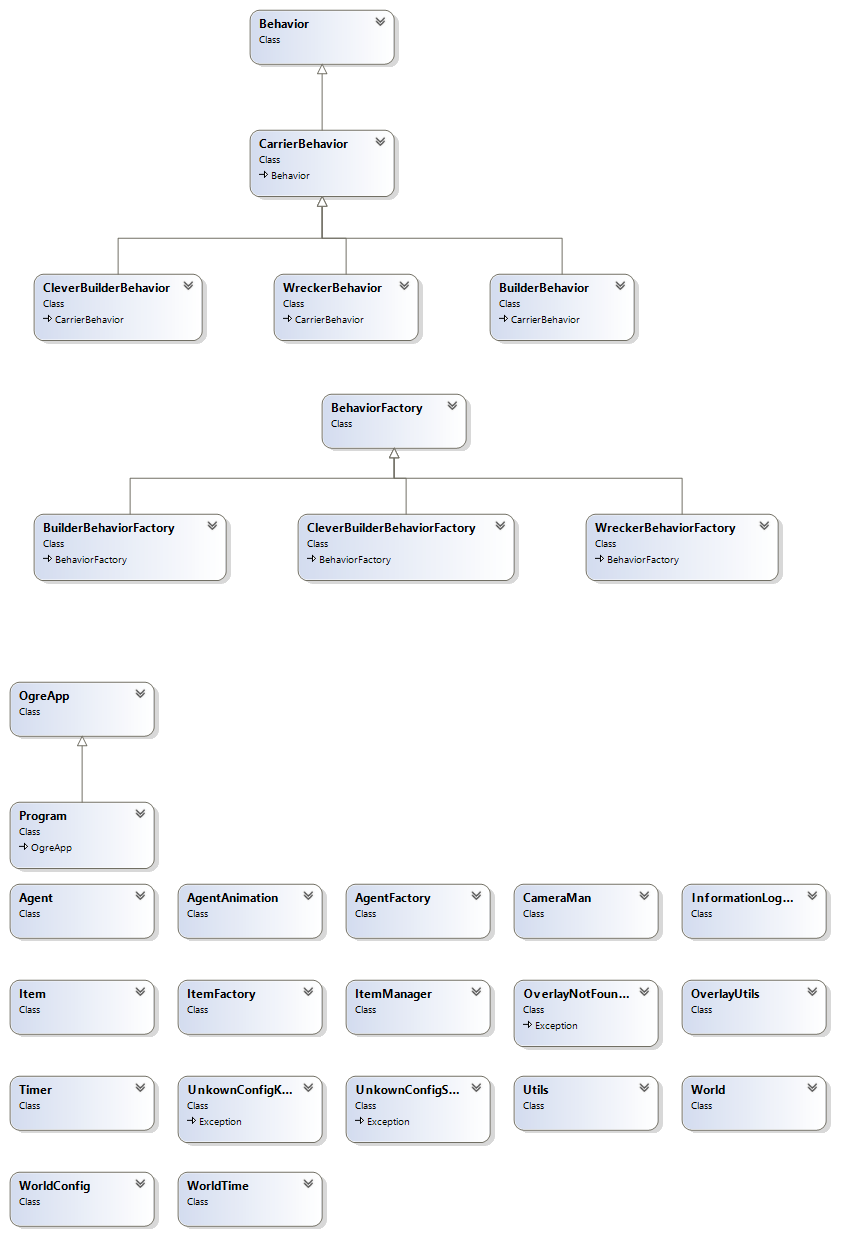
\includegraphics[width=15cm]{resources/ClassDiagram.png}
    \caption{Diagramme de classes du projet}
\end{figure}
